% !TEX program = xelatex
% 使用 texlive完整编译:
% xelatex -> bibtex -> xelatex -> xelatex
% 中文书籍 LaTeX 模板

%\PassOptionsToPackage{no-math}{fontspec}

\documentclass[UTF8,openany,twoside,12pt]{ctexbook}
%\documentclass[UTF8,openany,twoside,zihao=-4]{ctexbook}
%\documentclass[UTF8,twoside,12pt]{ctexbook}

%----- package for template -----
\usepackage{amsmath,amsthm,amssymb}
\usepackage{mathrsfs}
%\usepackage[notcite,notref]{showkeys}
%\usepackage[english]{babel}
\usepackage{imakeidx}
\usepackage{color,xcolor}
\usepackage{graphicx}
%\usepackage{epsfig}
\usepackage{tabularx,array}
\usepackage{longtable}
\usepackage{booktabs}
\usepackage{multirow}
\usepackage{multicol}
\usepackage{fancybox}
\usepackage{makecell}
\usepackage{xstring}
\usepackage{listings}
\usepackage{titletoc}
%\usepackage{titlesec}
\usepackage{caption}
\usepackage{mathtools}
\usepackage{float}
\usepackage[numbered]{bookmark}
\usepackage{anyfontsize}
%\usepackage{microtype}
\usepackage{geometry}
\geometry{left=2.5cm,right=2.5cm,top=3.0cm,bottom=3.0cm}
%\geometry{left=1in,right=1in,top=1in,bottom=1in}
%\geometry{left=2.5cm,right=2.1cm,top=1.7cm,bottom=2cm,includehead,includefoot}
%\geometry{b5paper,text={125mm,195mm},centering,left=1in,right=1in,top=1in,bottom=1in}
\setlength{\headheight}{18pt}
\setlength{\headsep}{18pt}
\setlength{\footskip}{25pt}

%\usepackage[title,titletoc]{appendix}
%\renewcommand{\appendixname}{附录}

%----- 设置超链接 -----
\usepackage{hyperref}
\hypersetup{
  colorlinks=true,
  linkcolor=black,
  citecolor=blue,
  filecolor=blue,
  urlcolor=blue,
}

%----- 设置英文字体 -----
%\usepackage[no-math]{fontspec}
%\usepackage{newtxtext}  % New TX font for text
%\setmainfont{TeX Gyre Termes}  % Times New Roman 的开源复刻版本
%\setsansfont{TeX Gyre Heros}   % Helvetica 的开源复刻版本
%\setmonofont{TeX Gyre Cursor}  % Courier New 的开源复刻版本
%\setmainfont{Times New Roman}
%\setsansfont{Arial}
%\setmonofont{Courier New}

%----- 设置数学字体 -----
%\usepackage{newtxmath}
%\usepackage{mathptmx}

%----- 直接插入 pdf 文件 -----
%\usepackage{pdfpages}

%----- 算法宏包及设置 -----
\usepackage{algorithm}
\usepackage{algpseudocode}
\floatname{algorithm}{算法}
\algrenewcommand\algorithmicrequire{\textbf{输入:}}
\algrenewcommand\algorithmicensure{\textbf{输出:}}

%----- 定义列表项的样式 -----
\usepackage{enumitem}
\setlist{nolistsep}
%\setlength{\itemsep}{3pt plus1pt minus2pt}

%\usepackage{indentfirst}  % 首行缩进宏包
%\usepackage[perpage,symbol]{footmisc}  % 脚注控制

%-----设置cleardoublepage-----
%\usepackage[cleardoublepage=plain]{scrextend}
\makeatletter
\renewcommand{\cleardoublepage}{\clearpage
  \clearpage\if@twoside\ifodd\c@page\else%
  \thispagestyle{empty}%
  \hbox{}\newpage\if@twocolumn\hbox{}\newpage\fi\fi\fi%
}
\makeatother

%----- 设置页眉和页脚 -----
\usepackage{fancyhdr,fancyref}
\pagestyle{fancy}
\fancyhf{}
\fancyhead[RO,LE]{\fangsong \zihao{5} ~\thepage~}
\fancyhead[LO]{\fangsong \zihao{5} \leftmark}
\fancyhead[RE]{\fangsong \zihao{5} \rightmark}
%\fancyhead[LO,RE]{\fangsong \zihao{5} \leftmark}
\lfoot{}
\cfoot{}
\rfoot{}

%----- 定义定理格式 -----
\newtheoremstyle{plain}
{0.5\topsep}{0.5\topsep}
{\itshape}{}{\bfseries}
{.}{5pt plus 1pt minus 1pt}{}
\theoremstyle{plain}
\newtheorem{definition}{定义}[chapter]
\newtheorem{proposition}{命题}[chapter]
\newtheorem{lemma}{引理}[chapter]
\newtheorem{theorem}{定理}[chapter]
\newtheorem{example}{例}[chapter]
\newtheorem{corollary}{推论}[chapter]
\newtheorem{remark}{注}[chapter]
\newtheorem{exercise}{练习}[chapter]
\newtheorem{assumption}{假设}[chapter]
\newtheorem{axiom}{公理}[chapter]
\newtheorem{property}{性质}[chapter]
\newtheorem{conjecture}{猜想}[chapter]
\renewcommand{\proofname}{\bfseries 证明}
\makeatletter
\renewenvironment{proof}[1][\proofname]{\par
  \pushQED{\qed}%
  %\normalfont \topsep6\p@\@plus6\p@\relax
  \normalfont \topsep0\p@\@plus3\p@\relax
  \trivlist
  \item[\hskip\labelsep\bfseries
  #1\@addpunct{\,:\,}]\ignorespaces
}{%
  \popQED\endtrivlist\@endpefalse
}
\makeatother

%-----设置图片的路径-----
\graphicspath{{./figure/}{./figures/}{./image/}{./images/}}

%----- 重新设置图表autoref -------
\renewcommand{\figureautorefname}{图}
\renewcommand{\tableautorefname}{表}

%----- 使用 tabularx库并定义新的左右中格式 -----
\newcolumntype{L}{X}
\newcolumntype{C}{>{\centering \arraybackslash}X}
\newcolumntype{R}{>{\raggedleft \arraybackslash}X}
\newcolumntype{P}[1]{>{\centering \arraybackslash}p{#1}}

%-----设置公式间距-----
\AtBeginDocument{
  \setlength{\abovedisplayskip}{6pt plus 2pt minus 2pt}
  \setlength{\belowdisplayskip}{6pt plus 2pt minus 2pt}
  \setlength{\abovedisplayshortskip}{3pt plus 1pt minus 1pt}
  \setlength{\belowdisplayshortskip}{3pt plus 1pt minus 1pt}
  %\setlength{\arraycolsep}{2pt}
}

%---------- 定义章节标题格式 ------------
\newcommand{\chapfont}{\fontsize{20pt}{20pt}\selectfont}
%--- chapter ---
\ctexset{
  chapter = {
    format = \linespread{1.0}\bfseries\chapfont\centering,
    name={第,章},
    nameformat = {},
    titleformat = {},
    number = \arabic{chapter},
    %number = \chinese{chapter},
    numberformat = {},
    aftername = \quad,
    beforeskip = {-4pt},
    afterskip = {24pt},
    pagestyle = plain,
  }
}
%--- section ---
\ctexset{
  section = {
    format = \linespread{1.0}\bfseries\zihao{-3}\raggedright,
    numberformat = {},
    aftername = \quad,
    beforeskip = {24pt},
    afterskip = {6pt},
  }
}
%--- subsection ---
\ctexset{
  subsection = {
    format = \linespread{1.0}\bfseries\zihao{4}\raggedright,
    numberformat = {},
    aftername = \quad,
    beforeskip = {12pt},
    afterskip = {6pt},
  }
}
%--- subsubsection ---
\ctexset{
  subsubsection = {
    format = \linespread{1.0}\bfseries\zihao{-4}\raggedright,
    numberformat = {},
    aftername = \quad,
    beforeskip = {12pt},
    afterskip = {6pt},
  }
}
%--- appendix ---
\ctexset{
  appendix = {
    name = {附录},
    numbering = true,
    number = \Alph{chapter},
  }
}

%\ctexset{
%chapter={name={第,章},number=\chinese{chapter}},
%section={name={{\bf\S}},number={\normalsize{\arabic{section}}}},
%subsection={number=\arabic{section}.\arabic{subsection}},
%}

%------------- 定义新的目录页面 ----------------
\usepackage{tocloft}
\renewcommand{\cfttoctitlefont}{\hfill \bfseries\chapfont}
%\renewcommand{\cftchappresnum}{第}
%\renewcommand{\cftchapaftersnum}{章}
\renewcommand{\contentsname}{目~~录}%\LARGE
\renewcommand{\cftaftertoctitle}{\hfill}
%\renewcommand{\cftchapaftersnumb}{\hspace{28pt}}
\setlength{\cftbeforetoctitleskip}{5pt}
\setlength{\cftaftertoctitleskip}{24pt}
\setlength{\cftbeforechapskip}{10pt plus 2pt minus 2pt}
\setlength{\cftbeforesecskip}{3pt}
\renewcommand{\cftdot}{$\cdot$}
\renewcommand{\cftdotsep}{3}
\renewcommand{\cftchapdotsep}{\cftdotsep}
\renewcommand\cftchapleader{\cftdotfill{\cftchapdotsep}}
\renewcommand{\cftsecdotsep}{\cftdotsep}  % 设置Section引导点

%--------- 定制图形和表格标题的样式 --------------
\captionsetup{font={small,singlespacing},labelformat={default},labelsep=quad}
\captionsetup[figure]{position=bottom,skip={5pt},name={图}}
\captionsetup[table]{position=top,skip={2pt},name={表}}
\setlength{\textfloatsep}{12pt plus 2pt minus 2pt}
\setlength{\floatsep}{10pt plus 2pt minus 2pt}
\setlength{\intextsep}{10pt plus 2pt minus 2pt}
\setlength{\abovecaptionskip}{2pt plus 1pt minus 1pt}
\setlength{\belowcaptionskip}{3pt plus 1pt minus 2pt}
%\setlength{\itemsep}{3pt plus 1pt minus 2pt}

\makeindex
%\bibliographystyle{plain}

\renewcommand{\baselinestretch}{1.35}        % 定义行距

%----- 参考文献格式 -----
%\bibliographystyle{plain} % abbrv, unsrt, siam
\bibliographystyle{thuthesis-numeric}
%\bibliographystyle{thuthesis-author-year}

%----- 参考文献引用格式 -----
\usepackage[numbers,sort&compress]{natbib}
%\usepackage[numbers,super,square,sort&compress]{natbib}
\def\bibfont{\small}  % 修改参考文献字体
\setlength{\bibsep}{7pt plus 3pt minus 3pt}  % 调整参考文献间距

%----- 微分符号 -----
\newcommand{\dif}{\mathop{}\!\mathrm{d}}

%----- 定义新命令 -----
\newcommand{\CC}{\ensuremath{\mathbb{C}}}
\newcommand{\RR}{\ensuremath{\mathbb{R}}}
\newcommand{\abs}[1]{\lvert#1\rvert}
\newcommand{\norm}[1]{\lVert#1\rVert}
\newcommand{\dx}[1][x]{\mathop{}\!\mathrm{d}#1}
\newcommand{\ii}{\mathrm{i}\mkern1mu} % imaginary
\newcommand{\refe}[2]{(\ref{#1})--(\ref{#2})}
\newcommand{\A}{\mathcal{A}}
\newcommand{\bA}{\boldsymbol{A}}
\newcommand{\red}[1]{\textcolor{red}{#1}}

% Generic dummy publisher logo
\newcommand{\plogo}{\fbox{$\mathcal{PL}$}}


%----- 书籍信息 -----
\title{\bfseries \LaTeX{} 书籍样例}
\author{\fangsong 某某某~~编著}
\date{\fangsong 202X年X月}


\begin{document}

%\maketitle  % 生成封面

%------- 自定义封面 -----------

\begin{titlepage}
  \makeatletter
  \pdfbookmark[0]{封~~面}{cover}
  \centering   % 将所有内容放在标题页的中心
  \vspace*{2\baselineskip}   % 页面顶部的空白

  %------------------------------------------------
  %   题目
  %------------------------------------------------

  \rule{\textwidth}{1.6pt}\vspace*{-\baselineskip}\vspace*{2pt}  % 粗水平线
  \rule{\textwidth}{0.4pt}   % 细水平线

  \vspace{0.75\baselineskip} % 标题上方的空白

  {\LARGE\bfseries \@title \par} % 题目

  \vspace{0.75\baselineskip} % 标题下方的空白

  \rule{\textwidth}{0.4pt}\vspace*{-\baselineskip}\vspace{3.2pt} % 细水平线
  \rule{\textwidth}{1.6pt}  % 粗水平线

  \vspace{2\baselineskip}   % 标题栏后的空白

  %------------------------------------------------
  %   作者
  %------------------------------------------------

  % {\scshape\Large 某某某  \quad 编著 \\}
  {\fangsong\large \@author}

  \medskip

  {\fangsong\large \@date}
  \makeatother

  %\vspace{2\baselineskip}

  %\textit{机构的名字 \\ 地点}

  \vfill % Whitespace between editor names and publisher logo

  %------------------------------------------------
  %   出版社
  %------------------------------------------------

  \plogo % Publisher logo

  \vspace{0.3\baselineskip} % Whitespace under the publisher logo

  202X % Publication year

  {\large publisher} % Publisher

\end{titlepage}

\thispagestyle{empty}

%%%%%%%%%%%%%%%%%%%%%%%%%%%%%%%%%%%%%%%%%%%%%%%%%%%%

\frontmatter

%%%%%%%%%%%%%%%%%%%%%%%%%%%%%%%%%%%%%%%%%%%%%%%%%%%%

\chapter{序}

这部分是序言这部分是序言这部分是序言这部分是序言这部分是序言这部分是序言这部分是序言这部分是序言这部分是序言这部分是序言这部分是序言这部分是序言这部分是序言这部分是序言这部分是序言这部分是序言这部分是序言这部分是序言这部分是序言这部分是序言这部分是序言这部分是序言这部分是序言这部分是序言这部分是序言这部分是序言这部分是序言这部分是序言这部分是序言这部分是序言这部分是序言这部分是序言这部分是序言这部分是序言这部分是序言这部分是序言这部分是序言这部分

\chapter{前~~言}

这部分是前言这部分是前言这部分是前言这部分是前言这部分是前言这部分是前言这部分是前言这部分是前言这部分是前言这部分是前言这部分是前言这部分是前言这部分是前言这部分是前言这部分是前言这部分是前言这部分是前言这部分是前言这部分是前言这部分是前言这部分是前言这部分是前言这部分是前言这部分是前言这部分是前言这部分是前言这部分是前言这部分是前言这部分是前言这部分是前言这部分是前言这部分是前言这部分是前言这部分是前言这部分是前言这部分是前言这部分是前言这部分


%%%%%%%%%%%%%%%%%%%%%%%%%%%%%%%%%%%%%%%%%%%%%%%%%%%%

\renewcommand\contentsname{目~~录}
\cleardoublepage
\phantomsection
\pdfbookmark[chapter]{\contentsname}{toc}
\tableofcontents

%%%%%%%%%%%%%%%%%%%%%%%%%%%%%%%%%%%%%%%%%%%%%%%%%%%%

\mainmatter   % 页码阿拉伯数字, 章节编号

%%%%%%%%%%%%%%% 正文内容从这里开始  %%%%%%%%%%%%%%%%%%


\chapter{引言}

\section{研究背景}

这是小四号的正文字体, 行间距 1.35 倍.

通过空一行实现段落换行, 仅仅是回车并不会产生新的段落.

自定义一个命令 \verb|\red{文字}| 可以\red{加红文字}, 在论文修改阶段方便标记.

这是一个引用的示例 \cite{Tadmor2012} 和 \cite{LiLiu1997,Adams2003,TreWei2014}.

这是中文与 English 混排. 标点统一使用英文的标点 (英文没有的除外). 这是一段文字这是一段文字这是一段文字这是一段文字这是一段文字. 这是一段文字这是一段文字这是一段文字这是一段文字这是一段文字这是一段文字这是一段文字这是一段文字这是一段文字这是一段文字这是一段文字这是一段文字这是一段文字这是一段文字这是一段文字.

\section{主要结论}

这是一大段文字这是一大段文字这是一大段文字这是一大段文字这是一大段文字这是一大段文字这是一大段文字这是一大段文字这是一大段文字这是一大段文字这是一大段文字这是一大段文字这是一大段文字这是一大段文字这是一大段文字这是一大段文字这是一大段文字这是一大段文字这是一大段文字这是一大段文字这是一大段文字.


\section{结构安排}

本文接下来的写作安排如下:

第二章, 我们介绍了 LaTeX 常用环境, 包括列表的使用、文献引用、数学公式、定理环境以及算法环境.

第三章, 对于差分方法数值求解微分方程, 给出了一个简短的示例.

第四章, 针对插图环境, 给出了单个图形居中放置、两个图形并排放置以及多个图形并排放置的示例.

第五章, 针对表格环境, 介绍了一些自定义命令, 并给出相应的表格插入示例.

最后是参考文献、附录和后记.



%%%%%%%%%%%%%%%% LaTeX 常用环境 %%%%%%%%%%%%%%%%

\chapter{LaTeX 常用环境}

\section{列表的使用}

这是一个计数的列表.
\begin{enumerate}%[label={\rm (\arabic*)}]%\roman
  \item 第一项
    \begin{enumerate}
      \item 第一项中的第一项
      \item 第一项中的第二项
    \end{enumerate}
  \item 第二项
  \item 第三项
\end{enumerate}

这是一个不计数的列表.
\begin{itemize}%[label={$\bullet$}]
  \item 第一项
  \begin{itemize}
    \item 第一项中的第一项
    \item 第一项中的第二项
  \end{itemize}
  \item 第二项
  \item 第三项
\end{itemize}


\section{文献引用}

参考文献可采用 BibTeX 或 BibLaTeX 的方式生成 (文献信息写在文件 \verb|reference.bib| 中), 参考文献的样式为 \verb|thuthesis-numeric| (对应的引用格式可选 \verb|numbers| 或  \verb|super|)和 \verb|thuthesis-author-year| (对应的引用格式 \verb|authoryear|), 符合国家标准《信息与文献参考文献著录规则》GB/T 7714-2015, 论文中引用和参考的文献必须列出. 参考文献序号按所引文献在论文中出现的先后次序排列. 引用文献应在论文中的引用处加注文献序号, 并加注方括弧.

文献引用示例 \cite{LiLiu1997} 和 \cite{Adams2003,Shen1994}.


\section{数学公式}

数学公式的使用请参考《一份(不太)简短的 \LaTeX~2$\varepsilon$ 介绍》 (lshort-zh-cn), 更多的数学符号参考 The Comprehensive LaTeX Symbol List (symbols-a4).

自定义命令表示的几个数学符号 $\RR$, $\CC$, $\A$, $\ii$, $\bA$. 微分符号 $\dif$ 以及 $\dx$, $\dx[t]$.

在文中行内公式可以这么写: $a^2+b^2=c^2$, 这是勾股定理, 它还可以表示为 $c=\sqrt{a^2+b^2}$, 还可以让公式单独一段并且加上编号
\begin{equation}\label{eq:trifun}
\sin^2{\theta}+\cos^2{\theta}=1.
\end{equation}
还可以通过添加标签在正文中引用公式, 如等式~\eqref{eq:trifun} 或者 \ref{eq:trifun}.

读者可能阅读过其它手册或者资料, 知道 LaTeX 提供了 eqnarray 环境. 它按照等号左边—等号—等号右边呈三列对齐, 但等号周围的空隙过大, 加上公式编号等一些 bug, 目前已不推荐使用. (摘自 lshort-zh-cn)

多行公式常用 align 环境, 公式通过 \verb|&| 对齐. 分隔符通常放在等号左边:
\begin{align}
a & = b + c \\
& = d + e.
\end{align}

align 环境会给每行公式都编号. 我们仍然可以用 \verb|\notag| 或 \verb|\nonumber| 去掉某行的编号. 在以下的例子,
为了对齐等号, 我们将分隔符放在右侧, 并且此时需要在等号后添加一对括号 \verb|{}| 以产生正常的间距:
\begin{align}
a ={} & b + c \\
={} & d + e + f + g + h + i + j \notag \\
& + m + n + o \\
={} & p + q + r + s.
\end{align}

如果不需要按等号对齐, 只需罗列数个公式, gather 将是一个很好用的环境:
\begin{gather}
a = b + c \\
d = e + f + g \notag \\
h + i = j
\end{gather}

align 和 gather 有对应不带编号的环境 align* 和 gather*.
对于 align, gather, align* 与 gather* 等环境, 若添加命令 \verb|\allowdisplaybreaks| 后 (已添加), 公式可以跨页显示.

多个公式组在一起公用一个编号, 编号位于公式的居中位置, amsmath 宏包提供了诸如 aligned、gathered 等环境, 与 equation 环境套用.

这个公式使用 aligned 环境 (\textbf{推荐使用})
\begin{equation}\label{eq:alignedEq}
\left\{\begin{aligned}
  &-\frac{{\dif}^{2} u}{\dif x^{2}}+\frac{\mathrm{d} u}{\dif x}=\pi^{2} \sin (\pi x)+\pi \cos (\pi x),\quad x \in [0,1], \\
  &u(0)=0,\quad u(1)=0.
\end{aligned} \right.
\end{equation}
其中方程的解析解为 $u=\sin(\pi x)$.

这个公式使用 array 环境
\begin{equation}\label{eq:arrayEq}
\left\{\begin{array}{l}
\displaystyle
-\frac{{\dif}^{2} u}{\dif x^{2}}+\frac{\dif u}{\dif x}=\pi^{2} \sin (\pi x)+\pi \cos (\pi x),\quad x \in [0,1], \\[6pt]
u(0)=0,\quad u(1)=0.
\end{array} \right.
\end{equation}

aligned 与 equation 环境套用, 公式间距自动调节, 如果有分式, 分式也是行间显示. 如果用 array 与 equation 环境套用, 需要手动调整公式行间距和行间显示.


\section{定理环境}

\begin{definition}\label{def:foo}
这是一个定义.
\end{definition}

\begin{proposition}\label{prop:foo}
这是一个命题.
\end{proposition}

\begin{lemma}[Lemma]\label{lmm:foo}
这是一个引理.
\end{lemma}

\begin{theorem}[Theorem]\label{thm:foo}
这是一个定理.
\end{theorem}
\begin{proof}
这是证明环境.
\end{proof}

\begin{corollary}\label{cor:foo}
这是一个推论.
\end{corollary}

\begin{proposition}[Proposition]
这是一个命题.
\end{proposition}

\begin{lemma}\label{lmm:convergence} {\rm (\textit{参考文献}\cite{LiLiu1997})}
假设单步法具有 $p$ 阶精度, 且増量函数 $\varphi(x_{n}, u_{n}, h)$ 关于 $u$ 满足 Lipschitz 条件
\begin{equation}\label{eq:conver1}
|\varphi(x, u, h)-\varphi(x, \bar{u}, h)| \leqslant L_{\varphi}|u-\bar{u}|.
\end{equation}
\end{lemma}

\begin{theorem}\label{thm:convergence}
假设单步法具有 $p$ 阶精度, 且増量函数 $\varphi(x_{n}, u_{n}, h)$ 关于 $u$ 满足Lipschitz 条件
\begin{equation}\label{eq:conver2}
|\varphi(x, u, h)-\varphi(x, \bar{u}, h)| \leqslant L_{\varphi}|u-\bar{u}|.
\end{equation}
\end{theorem}
\begin{proof}[\normalfont\bfseries 证明~\nopunct]
由引理 \ref{lmm:convergence} 和 \eqref{eq:alignedEq} 式可以推出以上结论.
\end{proof}

\begin{remark}\label{rem:remark}
这是一个 remark.
\end{remark}

\begin{example}
这是一个例子.
\end{example}


\section{算法环境}

如下是算法~\ref{alg:euclid}.
\begin{algorithm}[H]
\small
\caption{~Euclid's algorithm}\label{alg:euclid}
\begin{algorithmic}[1]
  \Procedure{Euclid}{$a,b$}\Comment{The g.c.d. of a and b}
  \State $r\gets a\bmod b$
  \While{$r\not=0$}\Comment{We have the answer if r is 0}
  \State $a\gets b$
  \State $b\gets r$
  \State $r\gets a\bmod b$
  \EndWhile\label{euclidendwhile}
  \State \Return $b$\Comment{The gcd is b}
  \EndProcedure
\end{algorithmic}
\end{algorithm}

如下是算法~\ref{alg:foo}, 算法宽度可以通过 minipage 宏包调节.

\begin{center}
\vspace{-2ex}
\begin{minipage}{.9\linewidth}
\begin{algorithm}[H]
\caption{~算法的名字}\label{alg:foo}
\begin{algorithmic}[1]
\Require input parameters A, B, C
\Ensure output result
\State some description 算法介绍
\For{condition}
  \State ...
  \If{condition}
    \State ...
    \Else
    \State ...
  \EndIf
\EndFor
\While{condition}
  \State ...
\EndWhile
\State \Return result
\end{algorithmic}
\end{algorithm}
\end{minipage}
\end{center}



%%%%%%%%%%%%%%%%%%%%%%%%%%%% 微分方程的数值方法 %%%%%%%%%%%%%%%%%%%%%%%

\chapter{微分方程的数值方法}

本章我们考虑具有以下微分方程:
\begin{equation}\label{eq:PDE}
\left\{\begin{aligned}
& L u=-\frac{{\dif}^{2} u}{\dif x^{2}}+\frac{\dif u}{\dif x}+q u=f, \quad a < x < b, \\
& u(a)=\alpha, \quad u(b)=\beta.
\end{aligned}\right.
\end{equation}
其中 $q, f$ 为 $[a,b]$ 上的连续函数, $q \geqslant 0$; $\alpha, \beta$ 为给定常数. 这是最简单的椭圆方程第一边值问题 .

问题 \eqref{eq:PDE} 存在唯一解 (参考文献 \cite{LiLiu1997}).


\section{有限差分方法}
在偏微分方程的数值解法中, 有限差分法数学概念直观, 推导自然, 是发展较早且比较成熟的数值方法. 由于计算机只能存储有限个数据和做有限次运算, 所以任何一种用计算机解题的方法, 都必须把连续问题 (微分方程的边值问題、初值问题等) 离散化, 最终化成有限形式的线性代数方程组.

\subsection{数值格式}
将区间 $[a,b]$ 分成 $N$ 等份, 分点为
\begin{equation*}
  x_{i} = a+ih, \quad i=0,1, \cdots, N,
\end{equation*}
其中 $h=(b-a)/N$. 于是我们得到区间 $I=[a,b]$ 的一个网格剖分. $x_i$ 称为网格的节点, $h$ 称为步长.

为了方便起见, 令 $q_{i}=q(x_{i})$, $f_{i}=f(x_{i})$. 方程 \eqref{eq:PDE} 的差分方程为
\begin{equation}\label{eq:difEqu}
  L_{h} u_{i}=-\frac{u_{i+1}-2 u_{i}+u_{i-1}}{h^{2}}+\frac{u_{i+1}-u_{i-1}}{h}+q_{i} u_{i}=f_{i},\quad 1 \leqslant j \leqslant N-1,
\end{equation}
其中 $L_{h}$ 为差分算子, $u_i$ 为 $u(x)$ 在 $x=x_i$ 处的近似解即差分解.

差分方程 \eqref{eq:difEqu} 对于 $i=1,2, \cdots, N-1$ 都成立, 加上边值条件 $u_{0}=\alpha, u_{N}=\beta$, 就得到如下线性方程组:
\begin{equation}\label{eq:fdm}
\left\{\begin{aligned}
& L_{h} u_{i}=-\frac{u_{i+1}-2 u_{i}+u_{i-1}}{h^{2}}+\frac{u_{i+1}-u_{i-1}}{2h}+q_{i} u_{i}=f_{i}, ~~ i=1, \cdots, N-1, \\
& u_{0}=\alpha, \quad u_{N}=\beta.
\end{aligned}\right.
\end{equation}


\subsection{矩阵形式}

定义向量 $\boldsymbol{u}$:
\begin{equation*}
  \boldsymbol{u}=(u_{1}, u_{2}, \cdots, u_{N-1})^{\mathrm{T}}.
\end{equation*}

差分格式可以写为矩阵形式:
\begin{equation*}
  \boldsymbol{A}\boldsymbol{u}=\boldsymbol{f}.
\end{equation*}
其中矩阵 $\boldsymbol{A}$、向量 $\boldsymbol{f}$ 的定义如下, 注意向量 $\boldsymbol{f}$ 的首尾元素已包含了 $x=a$ 和 $x=b$ 处的边界条件.
\begin{equation}\label{eq:matrix1}
\boldsymbol{A}=\begin{bmatrix}
\frac{2}{h^{2}}+q_{1} & \frac{1}{2h}-\frac{1}{h^{2}} &   &  &  \\[8pt]
 -\frac{1}{2h}-\frac{1}{h^{2}} & \frac{2}{h^{2}}+q_{2} & \frac{1}{2h}-\frac{1}{h^{2}}  & &  \\[8pt]
  &  &  &  &    \\
  &  \ddots  & \ddots  &  \ddots  &  \\[8pt]
  &  &  &  &    \\
  &   & -\frac{1}{2h}-\frac{1}{h^{2}} & \frac{2}{h^{2}}+q_{N-2}& \frac{1}{2h}-\frac{1}{h^{2}} \\[8pt]
  &  &  & -\frac{1}{2h}-\frac{1}{h^{2}} & \frac{2}{h^{2}}+q_{N-1}
\end{bmatrix}.
\end{equation}

上一个矩阵用了 \verb|bmatrix| 环境, 也可以使用 \verb|array| 环境.
\begin{equation}\label{eq:matrix2}
\boldsymbol{A}=\left[\begin{array}{cccccc}
\frac{2}{h^{2}}+q_{1} & \frac{1}{2h}-\frac{1}{h^{2}} &  &  &  \\[8pt]
 -\frac{1}{2h}-\frac{1}{h^{2}} & \frac{2}{h^{2}}+q_{2} & \frac{1}{2h}-\frac{1}{h^{2}}  & &  \\[8pt]
  &  &  &  &   \\
  &  \ddots  & \ddots & \ddots &  \\[8pt]
  &  &  &  &   \\
  &   & -\frac{1}{2h}-\frac{1}{h^{2}} & \frac{2}{h^{2}}+q_{N-2} & \frac{1}{2h}-\frac{1}{h^{2}} \\[8pt]
  &  &  & -\frac{1}{2h}-\frac{1}{h^{2}} & \frac{2}{h^{2}}+q_{N-1}
\end{array}\right].
\end{equation}


%%%%%%%%%%%%%%%%%% 插图环境 %%%%%%%%%%%%%%%%%%%%

\chapter{插图LaTeX环境}

\section{图的使用}

XeLaTeX 环境下可以插入 EPS、PDF、PNG、JPEG、BMP 格式的图片, 也可以用绘图包 (如 tikz 宏包) 直接在 \LaTeX 中绘制图形. 值得注意的是 figure 环境一个浮动体\index{浮动体}环境, LaTeX 不总是浮动体放在你想要的地方, 但是 LaTeX 总是保证浮动体的相对顺序, 所以对图片 \verb|\label| 和 \verb|\ref| 的交叉引用就显得尤为重要。

\section{插图示例}

插入一个图形并居中放置, 如图~\ref{fig:sinx}.
\begin{figure}[htp!]
  \centering
  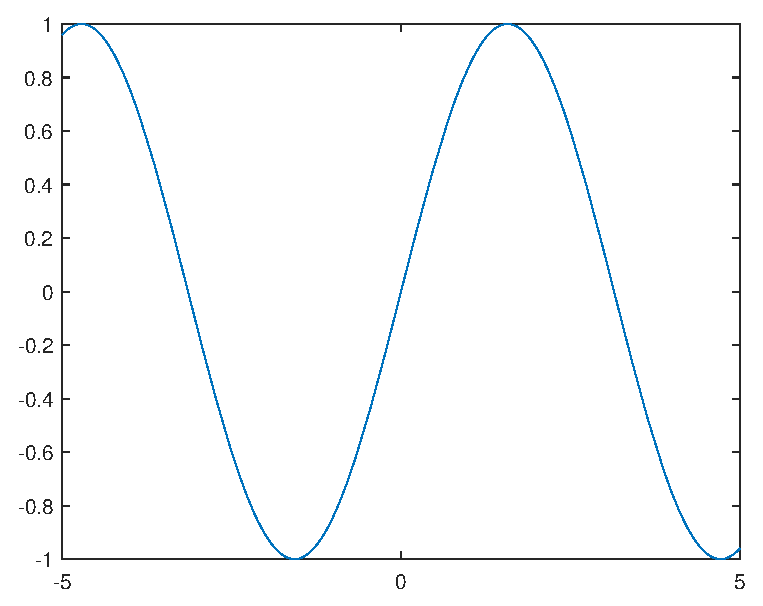
\includegraphics[width=7.2cm]{image1}
  \caption{函数 $y=\sin(x)$ 的图像}\label{fig:sinx}
\end{figure}

\clearpage
两个图左右并排放置, 共用一个标题, 如图~\ref{fig:twofigs}.
\begin{figure}[htp!]
  \centering
  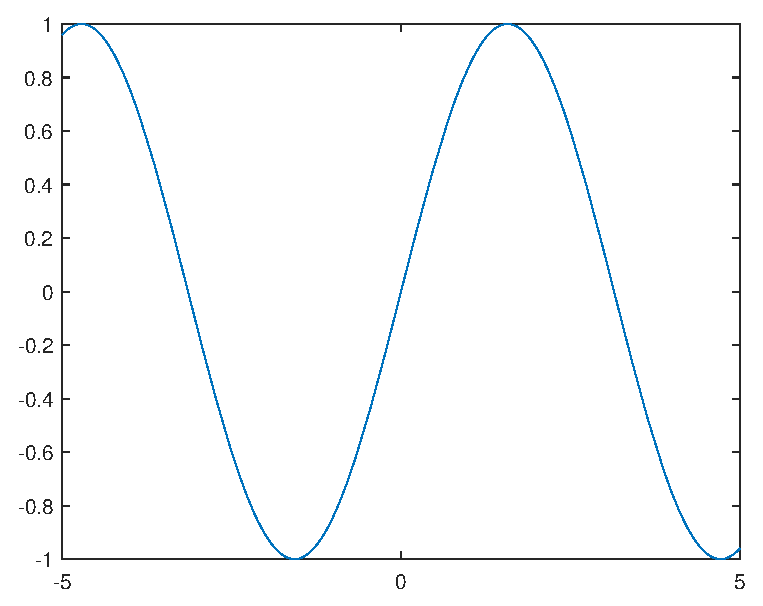
\includegraphics[width=0.45\linewidth]{image1}
  \hfill
  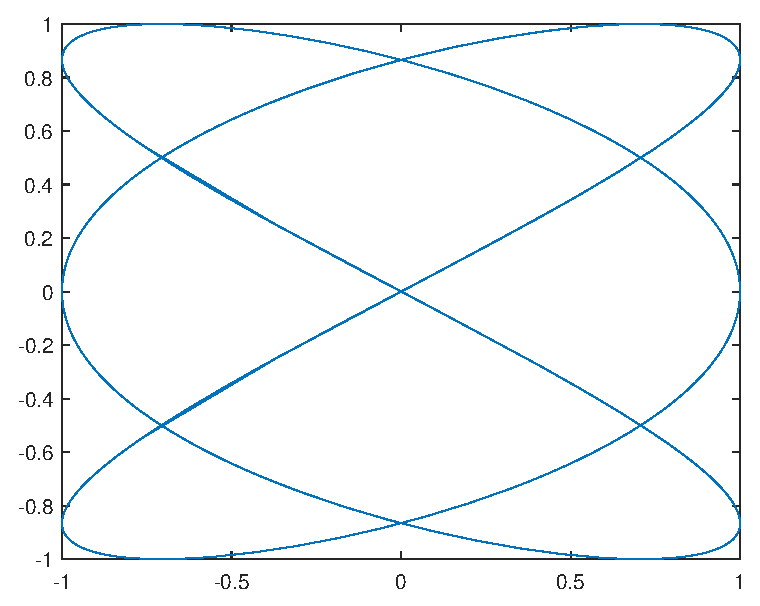
\includegraphics[width=0.45\linewidth]{image2}
  \caption{左: 图一的描述;~ 右:图二的描述.}
  \label{fig:twofigs}
\end{figure}


使用 minipage 排版并排插图, 每个图都有单独的标题. 通过 \verb|autoref| 引用图片: \autoref{fig:A} 与 \autoref{fig:B}.
\begin{figure}[htp!]
\begin{minipage}[t]{0.48\linewidth}
  \centering
  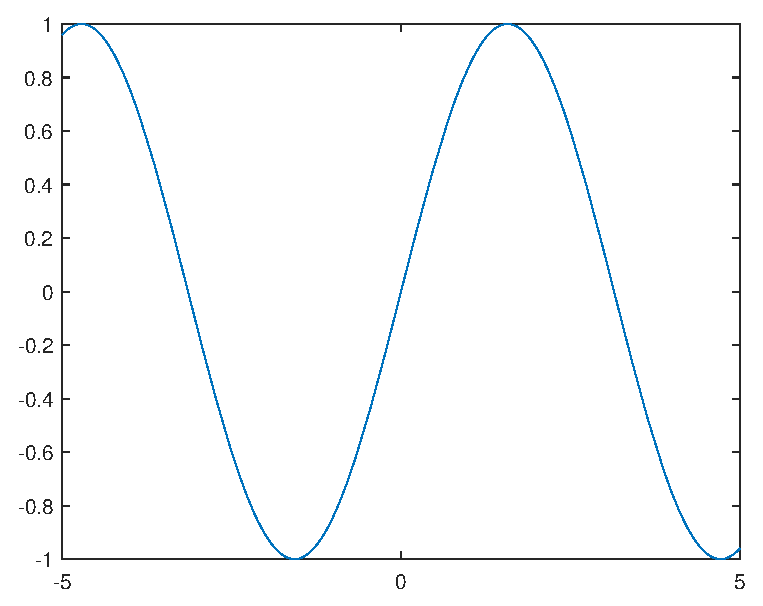
\includegraphics[width=0.9\linewidth]{image1}
  \caption{图一的描述.}
  \label{fig:A}
\end{minipage}
\hfill
\begin{minipage}[t]{0.48\linewidth}
\centering
  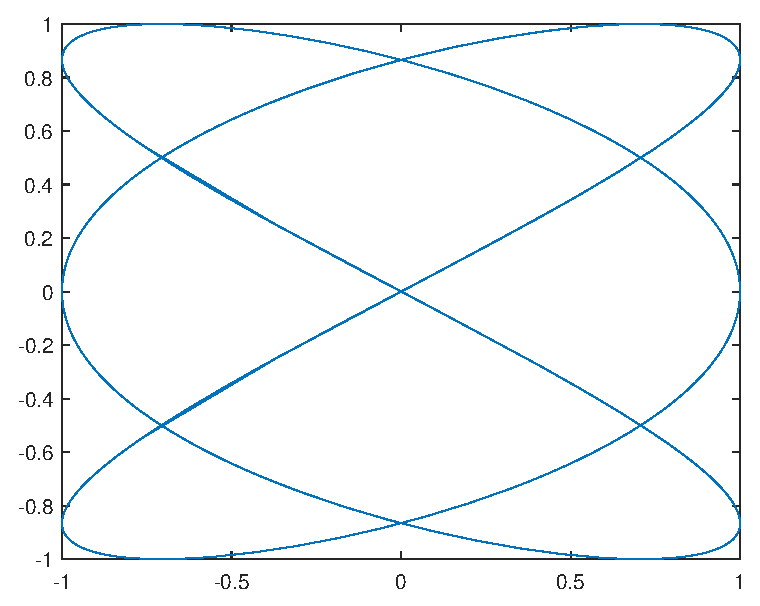
\includegraphics[width=0.9\linewidth]{image2}
  \caption{图二的描述.}
  \label{fig:B}
\end{minipage}
\end{figure}

%使用 subfig 宏包实现多图并排, 如图~\ref{fig:images}.
%\begin{figure}[htp!]
%\centering
%\subfloat[Subcaption A]{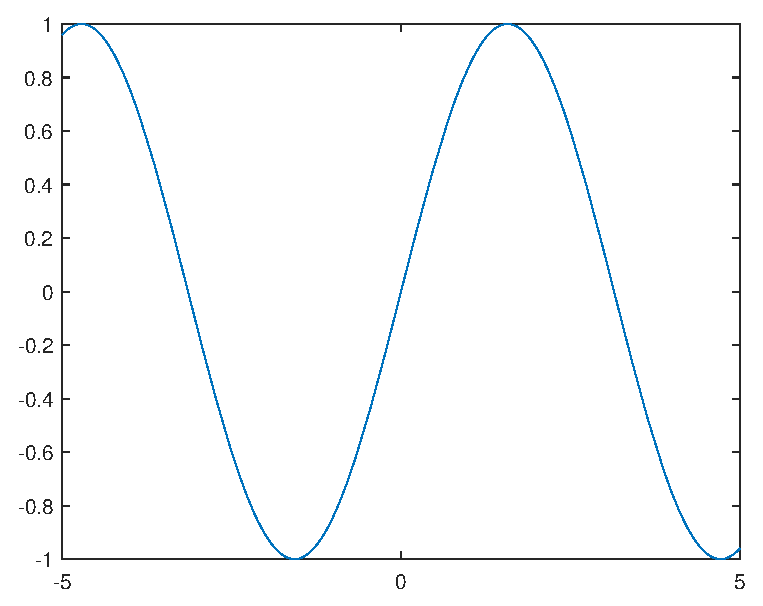
\includegraphics[width=0.3\linewidth]{image1}}
%\hfill
%\subfloat[Subcaption B]{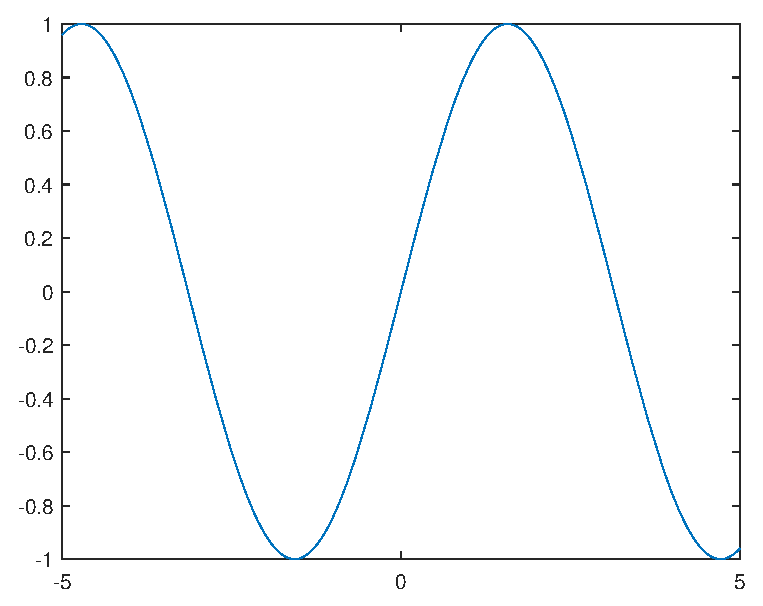
\includegraphics[width=0.3\linewidth]{image1}}
%\hfill
%\subfloat[Subcaption C]{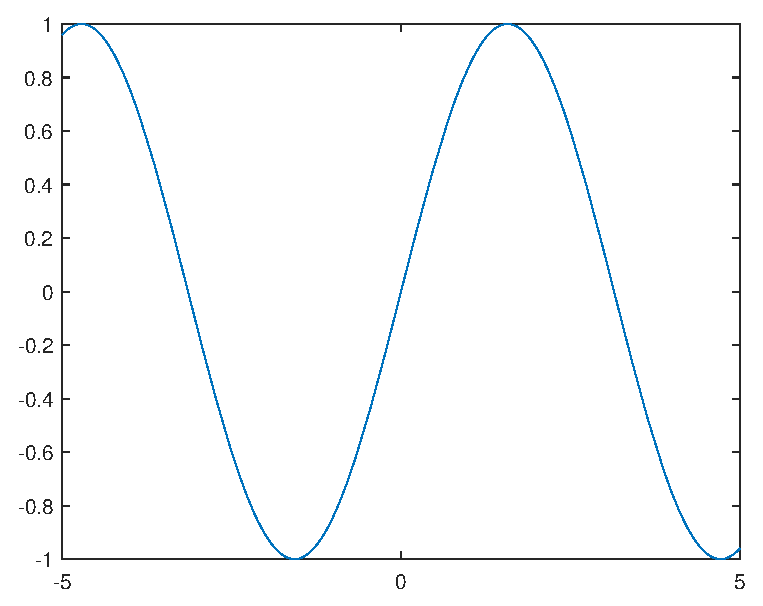
\includegraphics[width=0.3\linewidth]{image1}} \\
%\subfloat[Subcaption D]{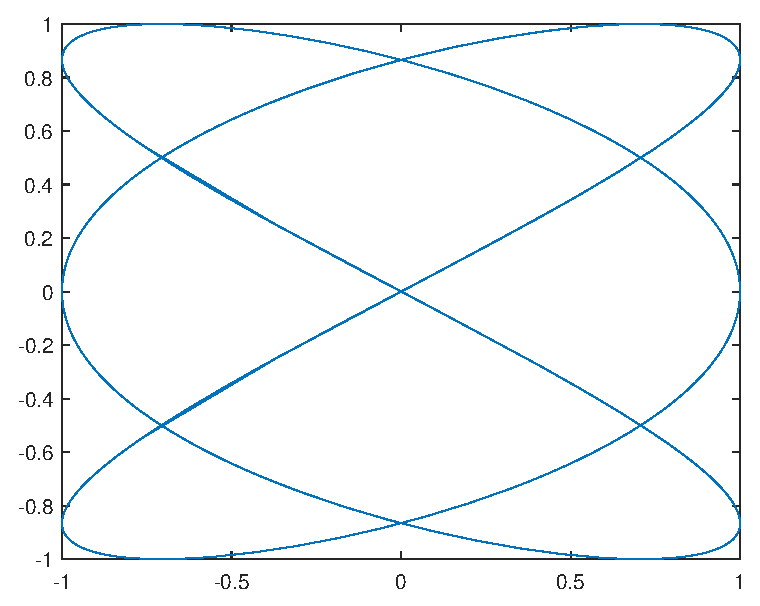
\includegraphics[width=0.3\linewidth]{image2}}
%\hfill
%\subfloat[Subcaption E]{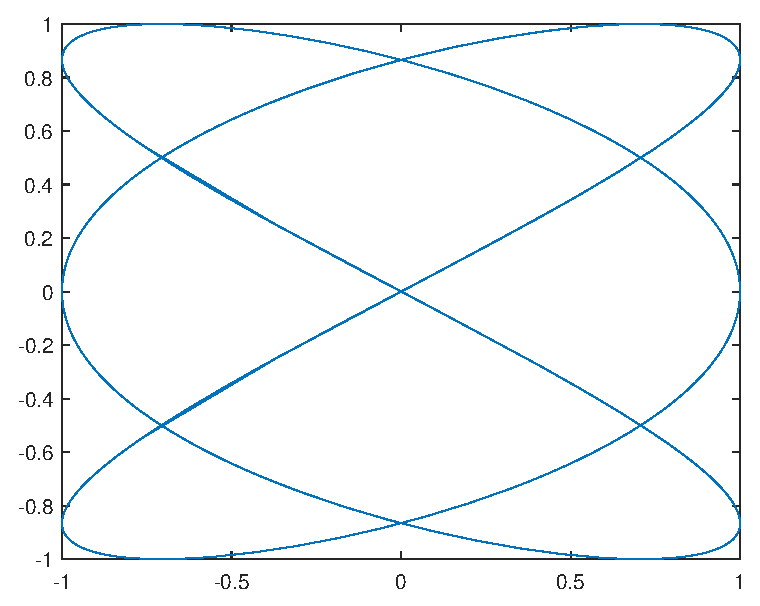
\includegraphics[width=0.3\linewidth]{image2}}
%\hfill
%\subfloat[Subcaption F]{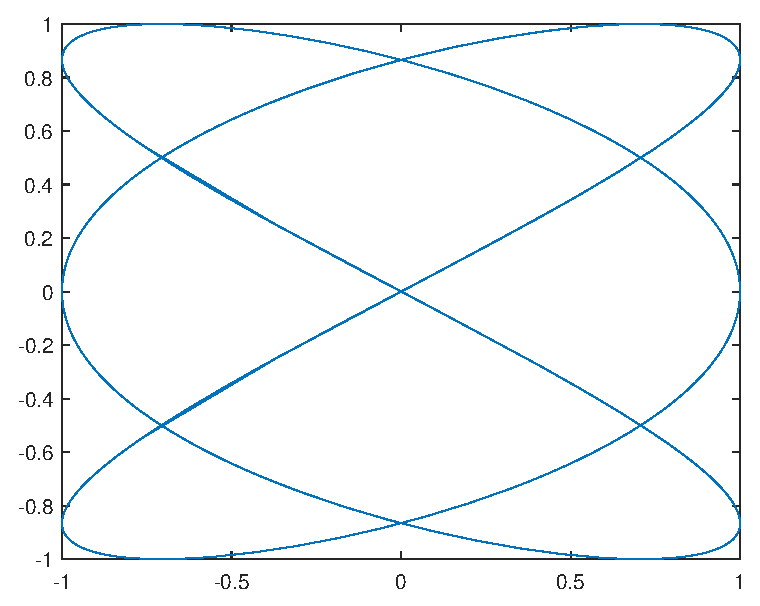
\includegraphics[width=0.3\linewidth]{image2}}
%\caption{六个图并排.}
%\label{fig:images}
%\end{figure}



%%%%%%%%%%%%%%%%%%% 表格环境 %%%%%%%%%%%%%%%%%%

\chapter{表格环境}

\section{表的使用}

LaTeX 的 table 环境是一个浮动体\index{浮动体}, 与 figure 环境的排版方式类似. 简单的表格可以使用三线表\index{三线表}进行排版, 其结构是仅在标题的上下以及表格的最下方添加横线.

排版表格最基本的环境是 tabular 环境, 适合大多数需求. 如果想要控制表格行列间距, 可使用命令 \verb|\tabcolsep| 和 \verb|\arraystretch|, 它们分别控制列间距和行间距. 例如, \verb|\tabcolsep{10pt}| 表示列间距为 10pt, 默认是 6pt,  \verb|\arraystretch{1.2}| 表示行间距为 1.2 倍, 默认是 1 倍间距.

本文基于 array 宏包定义了新的列类型 \verb|LCR| 格式, 实现了居左、居中和居右的对齐方式, 可用于 tabularx 环境. tabularx 环境要求先指定表格的总宽度, \verb|LCR| 三个格式根据表格的总宽度自动调整列宽, 使其相等. 本模板还定义了新的列类型 \verb|P{}|, 可用于 tabular 和 tabularx 环境, 它允许指定某列的宽度并使其内容居中 (如 \verb|P{1cm}| 控制某一列的宽度为 1cm), 实际上 \verb|P{}| 是在 \verb|p{}| 的基础上增加了居中功能.


\section{表格示例}

使用 tabular 环境, 如下表格: 表~\ref{tab:foo}. 通过 \verb|autoref| 引用表格: \autoref{tab:foo}.

\begin{table}[htp!]
\centering
\setlength{\tabcolsep}{12pt}  % 6pt standard
\renewcommand{\arraystretch}{1.2}
\caption{学术活动安排样例}
\label{tab:foo}
\begin{tabular}{|c|c|c|c|}
\hline
\textbf{日期} & \textbf{地点} & \textbf{活动名称} & \textbf{备注} \\ \hline
2024年8月1日     & 上海       & 学术研讨会     & 主题:人工智能 \\ \hline
2024年8月15日   & 北京      & 学术交流会      & 重点:数学建模 \\ \hline
2024年9月1日     & 深圳      & 研究研讨会      & 主题:数据科学 \\ \hline
2024年10月15日 & 广州      & 创新论坛          & 重点:科技创新 \\ \hline
\end{tabular}
\end{table}

使用 tabularx 环境, 如下表格: 表~\ref{tab:heightweight}.

\clearpage
\begin{table}[htp!]
\centering
% PLCR已经定义
\caption{某校学生身高体重样本}
\renewcommand\arraystretch{0.92}
\label{tab:heightweight}
\begin{tabularx}{0.9\textwidth}{P{1.5cm}CCC}
\toprule
序号 & 年龄 & 身高 & 体重 \\
\midrule
001 & 15 & 156 & 42 \\
002 & 16 & 158 & 45 \\
003 & 14 & 162 & 48 \\
004 & 15 & 163 & 50 \\
\cmidrule{2-4}
平均 & 15 & 159.75 & 46.25 \\
\bottomrule
\end{tabularx}
\end{table}


基于 tabular 环境设置一些格式: 上下表格线加粗, 如表~\ref{tab:error}.
\begin{table}[htp!]
%\small
\centering
%\setlength{\tabcolsep}{8pt}
%\renewcommand\arraystretch{1.1}
\caption{数值误差与收敛速率示例}
\label{tab:error}
\begin{tabular}{c|c|cc|cc|cc}
\Xhline{2\arrayrulewidth}
逼近次数 & 步长 $h$ & $L^2$ 误差 & 收敛阶 & $H^1$ 误差 & 收敛阶 & $L^\infty$ 误差 & 收敛阶 \\
\hline
  & 1/128 & 9.18E-06 & 2.02 & 7.70E-03 & 1.01  & 6.46E-07 & 2.02 \\
1 & 1/256 & 2.29E-06 & 2.01 & 1.92E-03 & 1.00  & 1.61E-07 & 2.01 \\
  & 1/512 & 5.70E-07 & 2.00 & 9.56E-04 & 1.00  & 4.01E-08 & 2.00 \\
\hline
  & 1/128 & 1.39E-08 & 3.01 & 1.15E-05 & 2.01  & 3.48E-12 & 4.02 \\
2 & 1/256 & 1.73E-09 & 3.01 & 2.88E-06 & 2.01  & 3.27E-13 & 3.94 \\
  & 1/512 & 2.17E-10 & 3.00 & 7.24E-06 & 2.00  & 6.66E-13 & 1.55 \\
\hline
  & 1/32  & 2.28E-09 & 4.05 & 6.92E-07 & 3.04  & 1.45E-15 & 8.21 \\
3 & 1/64  & 1.42E-10 & 4.03 & 8.65E-08 & 3.02  & 2.06E-14 & 3.85 \\
  & 1/128 & 8.91E-12 & 4.01 & 1.08E-08 & 3.01  & 3.86E-14 & 0.91 \\
\Xhline{2\arrayrulewidth}
\end{tabular}
\end{table}



%%%%%%%%%%%%%%%%% 生成参考文献 %%%%%%%%%%%%%%%%%%%%%

\clearpage
\phantomsection
\addcontentsline{toc}{chapter}{参考文献}

% 生成参考文献, 两种方式任选一种

% 第一种方式, 使用 bib 文件

%\nocite{*}  % 可以暂时显示全部参考文献
\bibliography{reference}


%------------------------------------------------

% 第二种方式, 手动添加文献信息

%\begin{thebibliography}{99}
%\bibitem{Tadmor2012} Tadmor~E. A review of numerical methods for nonlinear partial differential equations\allowbreak[J]. Bull. Amer. Math. Soc., 2012, 49(4): 507-554.
%
%\bibitem{LiLiu1997} 李荣华, 刘播. 微分方程数值解法\allowbreak[M]. 第四版. 北京: 高等教育出版社, 2009.
%
%\bibitem{Adams2003} Adams~R~A, Fournier~J~J~F. Sobolev spaces\allowbreak[M]. 2nd ed. Amsterdam: Elsevier, 2003.
%
%\bibitem{TreWei2014}Trefethen~L~N, Weideman~J~A~C. The exponentially convergent trapezoidal rule\allowbreak[J]. SIAM Rev., 2014, 56(3): 385-458.
%
%\bibitem{Shen1994} Shen~J. Efficient spectral-Galerkin method I. Direct solvers of second- and fourth-order equations using Legendre polynomials\allowbreak[J]. SIAM J. Sci. Comput., 1994, 15(6): 1489-1505.
%
%\end{thebibliography}



%%%%%%%%%%%%%%%%%%%%%%% 附录 %%%%%%%%%%%%%%%%%%%%%%%%

% 添加附录, 如不需要可以把附录部分注释
\appendix

% 附录正文
\chapter{这是第一个附录}

\section{附录A的小节}

这里是附录环境\index{附录环境}.

附录公式及编号
\begin{equation}\label{eq:abc}
  a^2+b^2=c^2.
\end{equation}

如图~\ref{fig:sinx2}.
\begin{figure}[htp!]
  \centering
  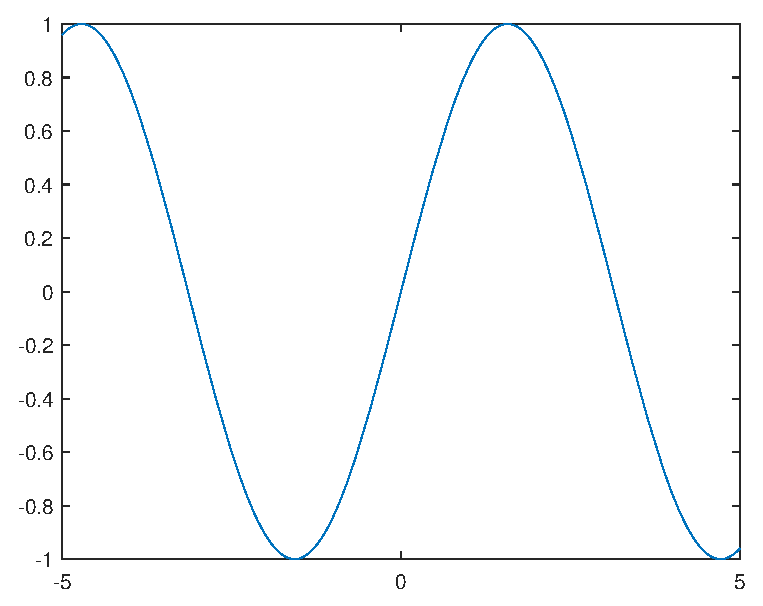
\includegraphics[width=0.45\linewidth]{image1}
  \caption{函数 $y=\sin(x)$ 的图像}\label{fig:sinx2}
\end{figure}


如下表格: 表~\ref{tab:heightweight2}.

\begin{table}[htp!]
\centering
% PLCR已经定义
\caption{某校学生身高体重样本.}
\label{tab:heightweight2}
\begin{tabularx}{0.9\textwidth}{P{1.5cm}CCC}
\toprule
序号 & 年龄 & 身高 & 体重\\
\midrule
001 & 14 & 156 & 42 \\
002 & 16 & 158 & 45 \\
003 & 14 & 162 & 48 \\
004 & 15 & 163 & 50 \\
\cmidrule{2-4}
平均 & 15 & 159.75 & 46.25 \\
\bottomrule
\end{tabularx}
\end{table}

\chapter{这是第二个附录}

\section{附录B的小节}

这里是附录环境.

内容附录内容附录内容附录内容\index{内容}附录内容附录内容附录内容附录内容附录内容附录内容附录内容附录内容附录内容附录内容附录内容附录内容附录内容附录内容附录内容附录内容附录内容正文内容正文. 内容附录内容附录内容附录内容附录内容附录内容附录内容附录内容附录内容附录内容附录内容附录内容附录内容附录内容附录内容附录内容附录内容附录内容文内容正文内容正文内容正文内容.



%%%%%%%%%%%%%%%%%%%%%%%%%%%%%%%%%%%%%%%%%%%%%%%%%%%%

\backmatter  % 结束章节自动编号

%%%%%%%%%%%%%%%%%%%%%%%%%%%%%%%%%%%%%%%%%%%%%%%%%%%%

%%%%%%%%%%%%%%%%%%%%% 索引  %%%%%%%%%%%%%%%%%%%%%%%%%

\clearpage
\renewcommand\indexname{索~~引}
\phantomsection
\addcontentsline{toc}{chapter}{索~~引}
\printindex


%%%%%%%%%%%%%%%%%%%%% 后记  %%%%%%%%%%%%%%%%%%%%%%%%%


\chapter{后~~记}

后记内容后记内容后记内容后记内容后记内容后记内容后记内容后记内容后记内容后记内容后记内容后记内容后记内容后记内容后记内容后记内容后记内容后记内容后记内容后记内容后记内容后记内容后记内容后记内容后记内容后记内容后记内容后记内容后记内容后记内容后记内容后记内容后记内容后记内容后记内容后记内容后记内容后记内容后记内容后记内容后记内容后记内容后记内容后记内容后记内容后记内容后记内容后记内容后记内容后记内容后记内容后记内容后记内容后记内容后记内容后记内容后记内容后记内容后记内容后记内容后记内容后记内容后记内容后记内容后记内容后记内容后记内容后记内容后记内容


\vspace{5ex}
\begin{flushright}
作~~者~~~~~~~~~

202X年X月~~~~~
\end{flushright}



\end{document}


